\TUchapter{Case Study: Caterpillar}

The approach described in Chapter 3 was tested against ECMs manufactured by Caterpillar, Inc. This manufacturer was
chosen for several reasons. Firstly, the process for extracting data from Caterpillar ECMs is unusually tedious compared
to other manufacturers' products, so automating it would provide maximum value to investigators.
Secondly, as will be explained shortly, the proprietary communications protocol used
by Caterpillar is encrypted in such a way that implementing a replay mechanism is challenging.

\TUsection{Caterpillar Data}

The information stored on the CAT ECMs under study include warranty report information and snapshot
information. The warranty report contains the identity of the ECM, historical usage information such as engine use histogram,
logged fault codes, and engine configuration information.

``Snapshots'' are a freeze-frame of the state of the truck at the time a critical fault is detected. These snapshots
include everything from wheel speed to engine speed. A bench download can lead to new snapshots being created, because an ECM that is outside
of a vehicle will interpret the lack of sensor data from a truck as a series of faults. As Caterpillar ECMs are typically
limited to four snapshots, creating new snapshots can overwrite existing snapshot information. As such, logging and replaying snapshot information is critical to any forensic solution for
Caterpillar ECMs.

\TUsection{Deciphering Network Data}

Observation of RP1210 calls made by the Caterpillar Electronic Technician (CAT ET) software showed that all requests sent by,
and all responses to those requests, were made using extensions to the J1708/J1587 and J1939 protocols
proprietary to Caterpillar. As requests and responses changed significantly between extractions, with
no change in data displayed, it was determined that some session-based encryption mechanism was
used.

\TUsubsection{Static Analysis}

As most of the CAT ET software is written using Microsoft's .NET framework, the software was decompiled
using JetBrains Software's dotPeek .NET decompiling tool. After some exploration of the code base,
the list of proprietary J1708 PIDs shown in Table \ref{tab:catet} was found.

\begin{table}[h]
  \centering
   \begin{tabular}{|c|c|}
    \hline
    Opcode & Function \\
    \hline
    0x70 & ReadRequest \\
    \hline
    0x80 & WriteRequest \\
    \hline
    0x90 & ReadWriteResponse\\
    \hline
    0xA0 & EncryptedBroadcastRequest\\
    \hline
    0xB0 & EncryptedBroadcastResponse\\
    \hline
    0xC0 & EncryptedReadRequest\\
    \hline
    0xD0 & EncryptedWriteRequest\\
    \hline
    0xE0 & EncryptedReadWriteResponse\\
    \hline
    0xF0 & SecuritySetup\\
    \hline
   \end{tabular}

\caption{Caterpillar ATA Function Codes}
\label{tab:catet}
\end{table}

The names of the functions obviously suggest that much of the message traffic is encrypted. Further analysis of the
decompiled code, and the disassembly of a native DLL,  revealed the following system:

\begin{enumerate}
  \item CAT ET sends a session key to the ECM using a SecuritySetup message.
  \item The ECM sends a session key to CAT ET using a SecuritySetup message.
  \item For each encrypted message, an individual key is generated by summing the
        current session key and the second nibble of the proprietary PID.
  \item Each message is passed to a native DLL along with its key for decryption.
  \item The key is an index into an array of bytes; the relevant byte is XOR'd
        with each byte in the message to encrypt/decrypt it.
\end{enumerate}


\begin{figure}[h]
  \centering
  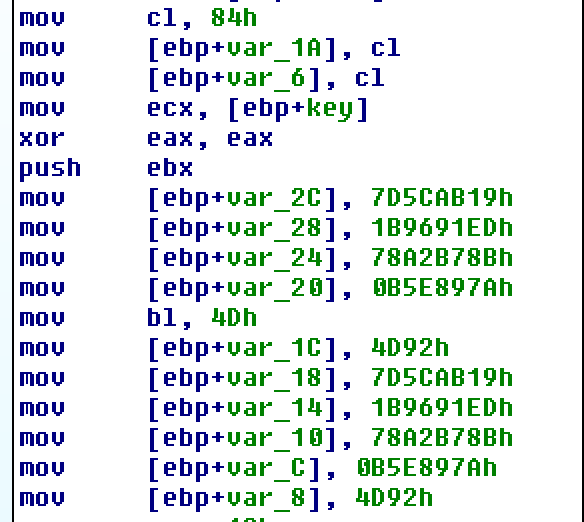
\includegraphics{CryptoKeysScreenshot}
  \caption{Disassembly showing decryption/encryption keys}
  \label{fig:atacryptkeys}
\end{figure}

\begin{figure}[h]
  \centering
  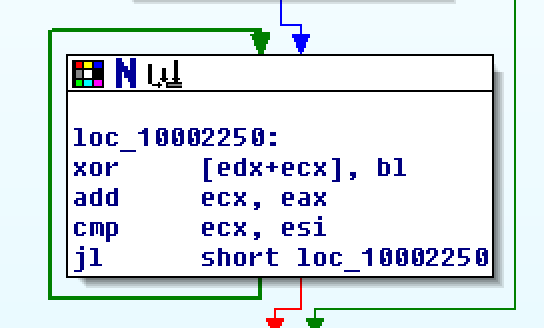
\includegraphics{CryptoAlgorithmScreenshot}
  \caption{Dissasembly showing decryption/encryption process}
  \label{fig:atacryptalgorithm}
\end{figure}


\TUsubsection{Dynamic Analysis}

Now that the algorithm that encrypted ECM communications was known, the information contained in those
messages could be observed to determine how that information should be extracted and replayed. The
API hooking tool described in Chapter 3 was extended to decrypt ECM communications on-the-fly
and log them when they were intercepted. It was discovered that the protocols followed the format depicted
in Figure \ref{fig:ataprotocol}

\begin{figure}[h]
  \centering
  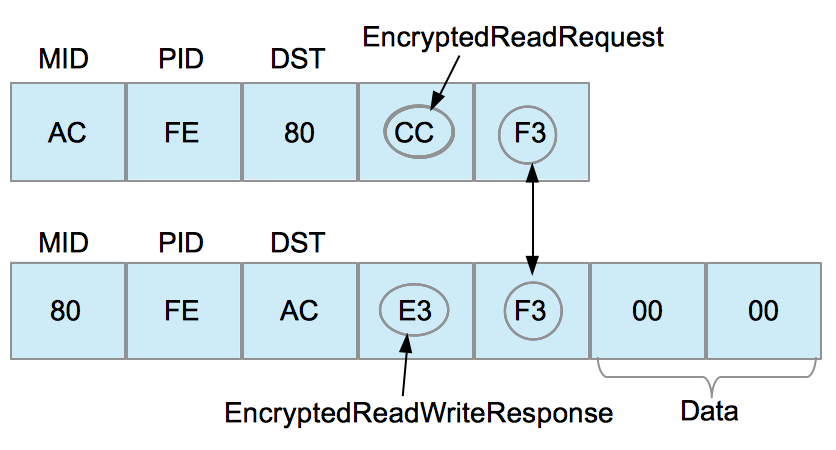
\includegraphics[scale=0.75]{cat-protocol-diagram}
  \caption{Example exchange in CAT ATA protocol}
  \label{fig:ataprotocol}
\end{figure}

\TUsection{Information Extraction}

Now that the mechanism of the protocol was somewhat understood, it was possible to extract the information.
A manual extraction was performed according to a checklist for a crash information extraction, and the 
RP1210 API calls were logged.

Each request was logged in a plaintext format as it was sent. 
It should be noted that the storage format preserves the opcode of the message. After the message was sent, proprietary
responses with matching PIDs were recorded in the key-value pair. It was observed that some responses were split over
several messages, so this was accounted for in the extraction software.

\TUsection{Verification}

In order to ensure that the method of information extraction was reliable, replays from the ECM were tested against
actual extractions from CAT ECMs.

\TUsubsection{Procedure}

The ECMs tested were evidence ECMs that were already used, and thus had been pre-populated with data.
The verification procedure was designed to determine the fidelity of the information replayed, as well as the
consistency of multiple replays of recorded data as compared to the consistency of multiple downloads of an
evidence ECM. The test procedure also aimed to test the generality of the specific ECM replay method derived
for Caterpillar ECMs by performing the same test against multiple ECMs.

\begin{figure}[h]
  \centering
  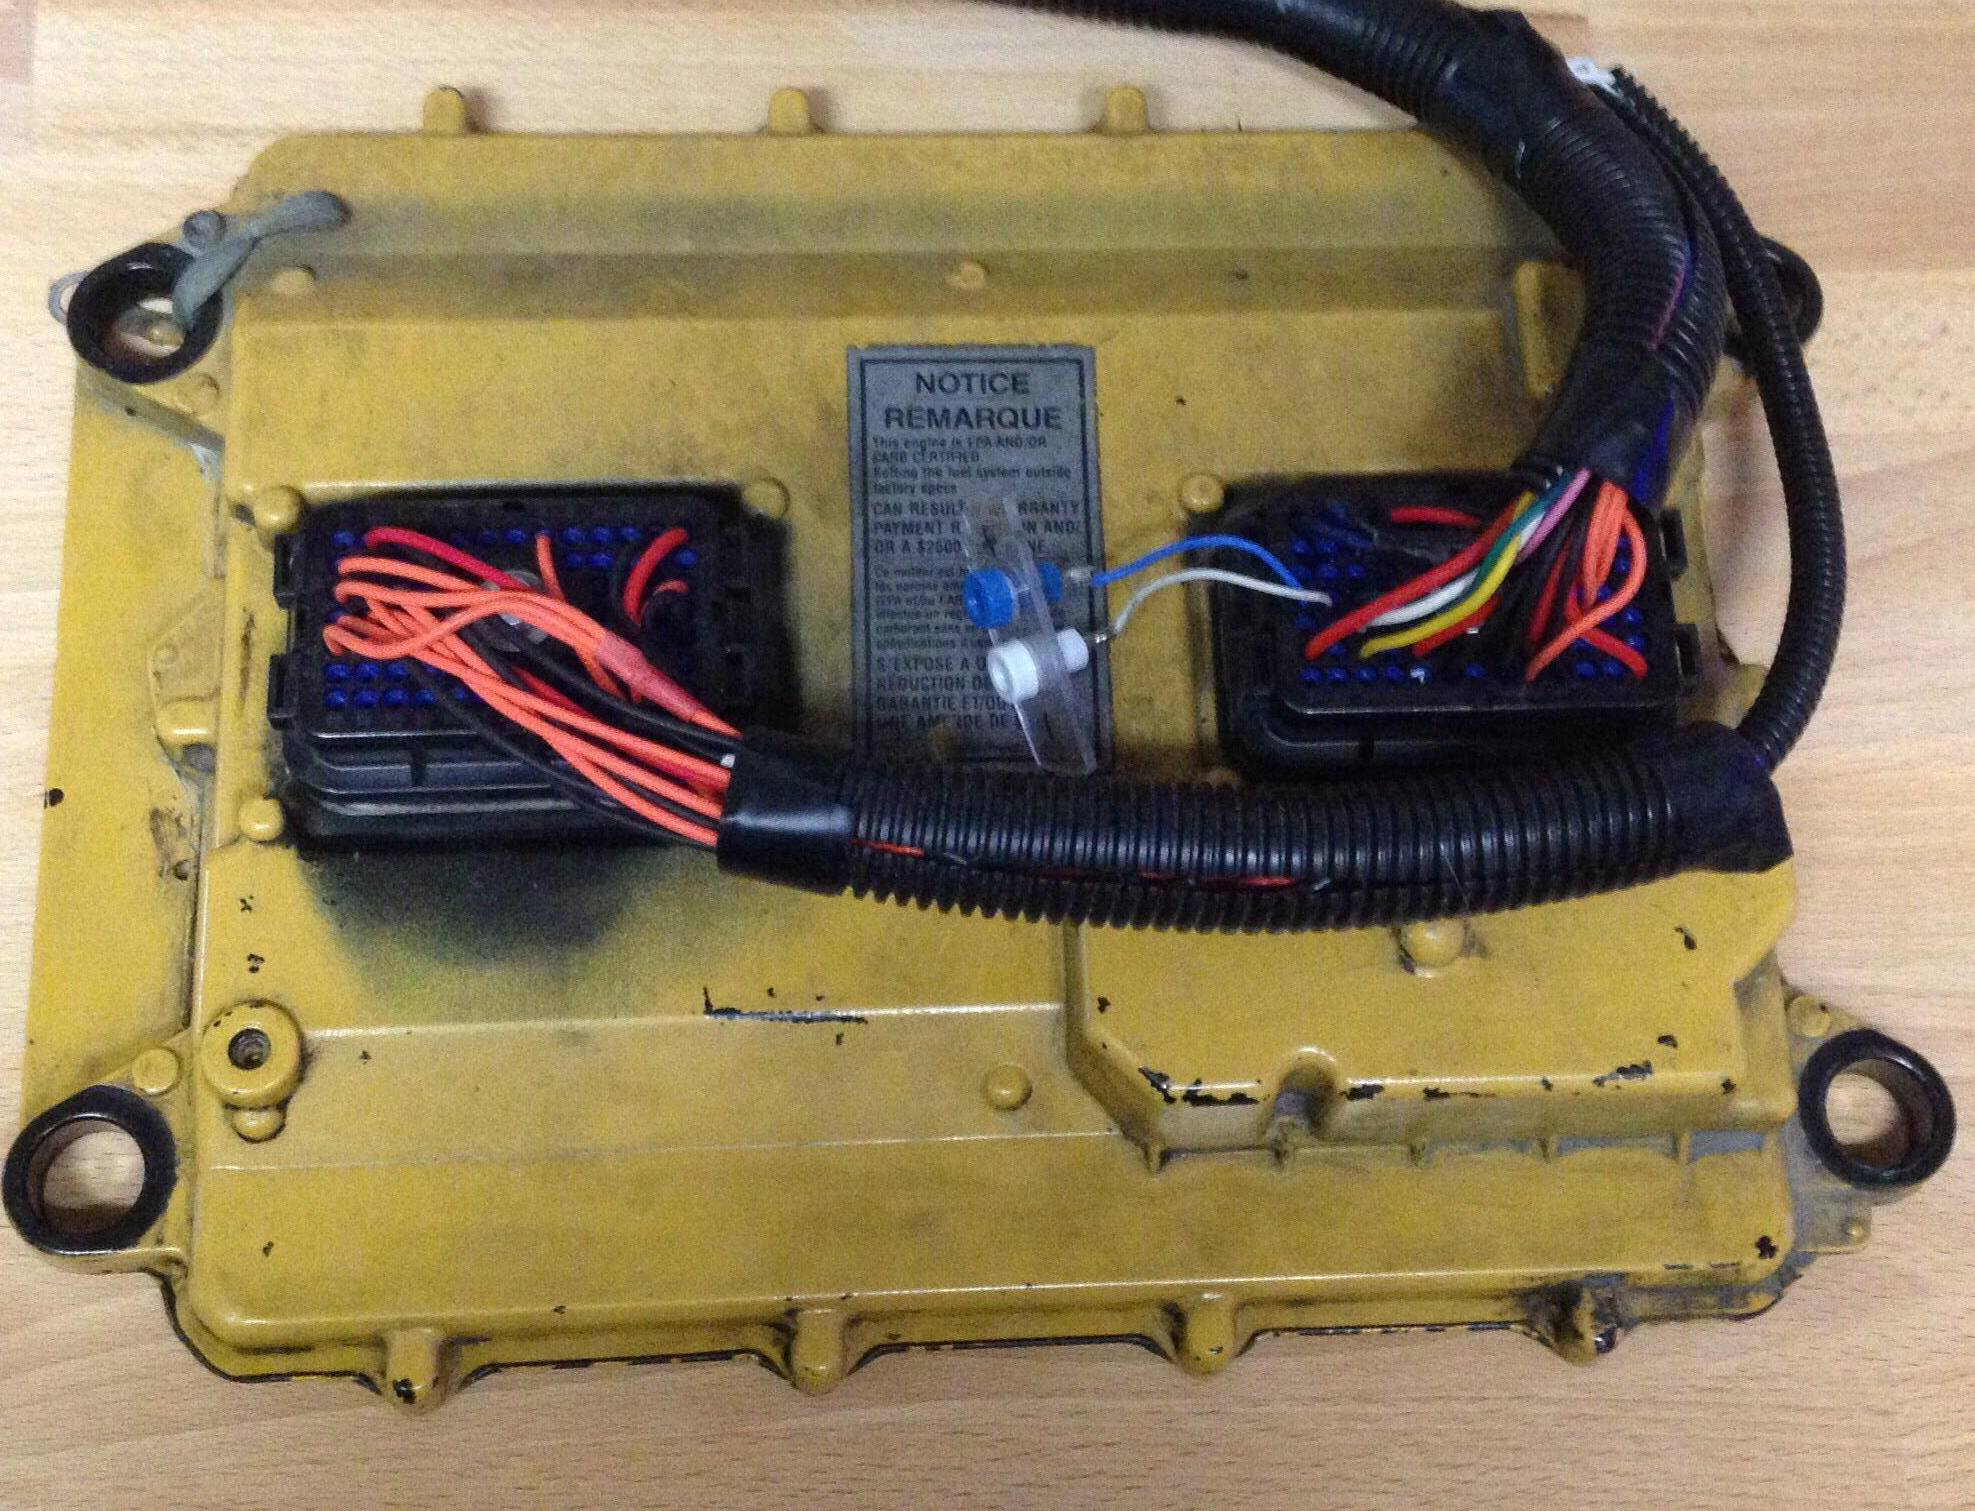
\includegraphics[scale=.2]{cat-ecm-1}
  \caption{First ECM for which replay was developed.}
  \label{fig:cat-ecm-1}
\end{figure}

\begin{figure}[h]
  \centering
  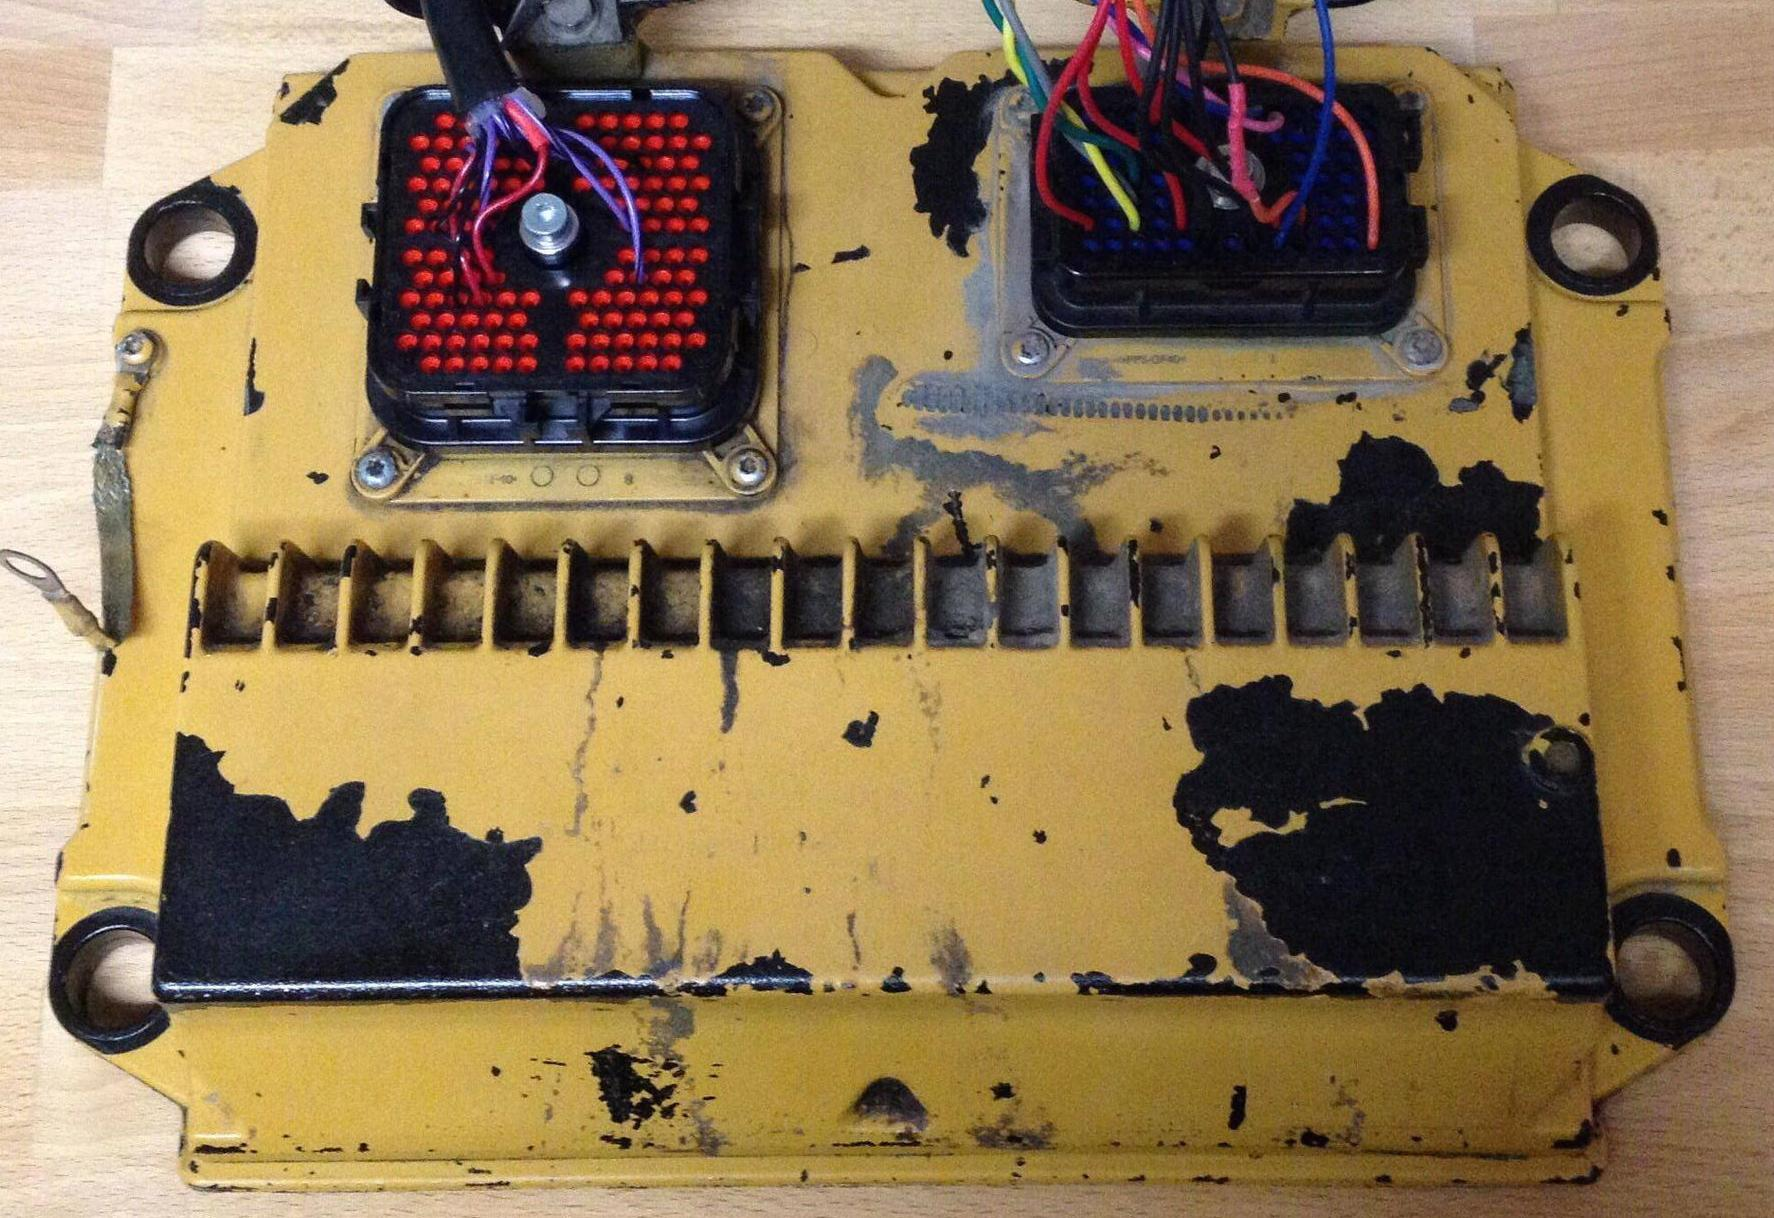
\includegraphics[scale=.2]{cat-ecm-2}
  \caption{Second test ECM, a CAT ADEM IV}
  \label{fig:cat-ecm-2}
\end{figure}


The steps of the test procedure were as follows:

\begin{enumerate}
  \item Perform one extraction of test ECM according to a checklist obtained from an accident reconstructionist while recording API calls. Save Warranty Report information and record snapshot information.
  \item Repeat step one twice more, each time saving Warranty Reports and recording snapshots.
  \item Extract ECM data using logged RP1210 calls obtained in step 1.
  \item Perform 3 replayed extractions, using data extracted in step 3.
  \item Compare ECM extractions to find differences in data contained therein.
  \item Compare replayed extractions to find differences in data.
  \item Compare consistency of ECM extractions and replayed extractions.
\end{enumerate}

\TUsubsection{Results}

Upon comparison, snapshots recorded from replayed traffic were identical to those recorded from identical ECM traffic. Warranty report information was also identical
between replayed traffic extractions. ECM running time figures changed from extraction to extraction when extracting data directly from the ECM; in this case, the
data extracted from the replay mechanism were more consistent than that from the ECM.


